\setbeamertemplate{itemize subitem}[triangle] % Pour le deuxième niveau
\setbeamertemplate{itemize subsubitem}[square] % Pour le troisième niveau
%\setbeamerfont*{itemize item}{size=\scriptsize}
\setbeamercolor{itemize item}{}
\setbeamercolor{itemize subitem}{fg=orange}
\setbeamercolor{itemize subsubitem}{fg=orange}

\setbeamerfont{headline}{size=\Large}\section{Results:}

%%

\section{{1-sample} estimation of correlation}
\protect\hypertarget{estimation-of-rho-one-sample}{}


\begin{frame}{squareEM iterations (n=1000)}

\begin{table}[htbp]
  \centering\scriptsize
  \begin{tabular}{*{2}{l}*{3}{r}}
    \toprule
    cs & \( \rho \) \textbar\ beta2 & \multicolumn{1}{c}{0} & \multicolumn{1}{c}{0.5} & \multicolumn{1}{c}{1} \\
    \midrule
    1 & -0.5 & 36 & 95 & 93 \\
    & -0.25 & 83 & 107 & 154 \\
    & 0 & 107 & 142 & {\color{red}250} \\
    & 0.25 & 90 & 127 & {\color{red}250} \\
    & 0.5 & 112 & 227 & {\color{red}250} \\ \addlinespace[3pt]
    0.8 & -0.5 & 36 & 90 & 116 \\
    & -0.25 & 88 & 108 & 243 \\
    & 0 & 119 & 163 & {\color{red}250} \\
    & 0.25 & 146 & 219 & {\color{red}250} \\
    & 0.5 & 141 & 248 & {\color{red}250} \\ \addlinespace[3pt]
    0.6 & -0.5 & 78 & 105 & {\color{red}250} \\
    & -0.25 & 117 & {\color{red}250} & 235 \\
    & 0 & 134 & 212 & {\color{red}250} \\
    & 0.25 & 159 & 240 & {\color{red}250} \\
    & 0.5 & 184 & {\color{red}250} & {\color{red}250} \\
    \bottomrule
  \end{tabular}
  \caption*{max number iterations to converge, nsim=100}
  \label{tab:ft1b}
\end{table}
\end{frame}




\begin{frame}{Correlation (n=100)}

\begin{center}
  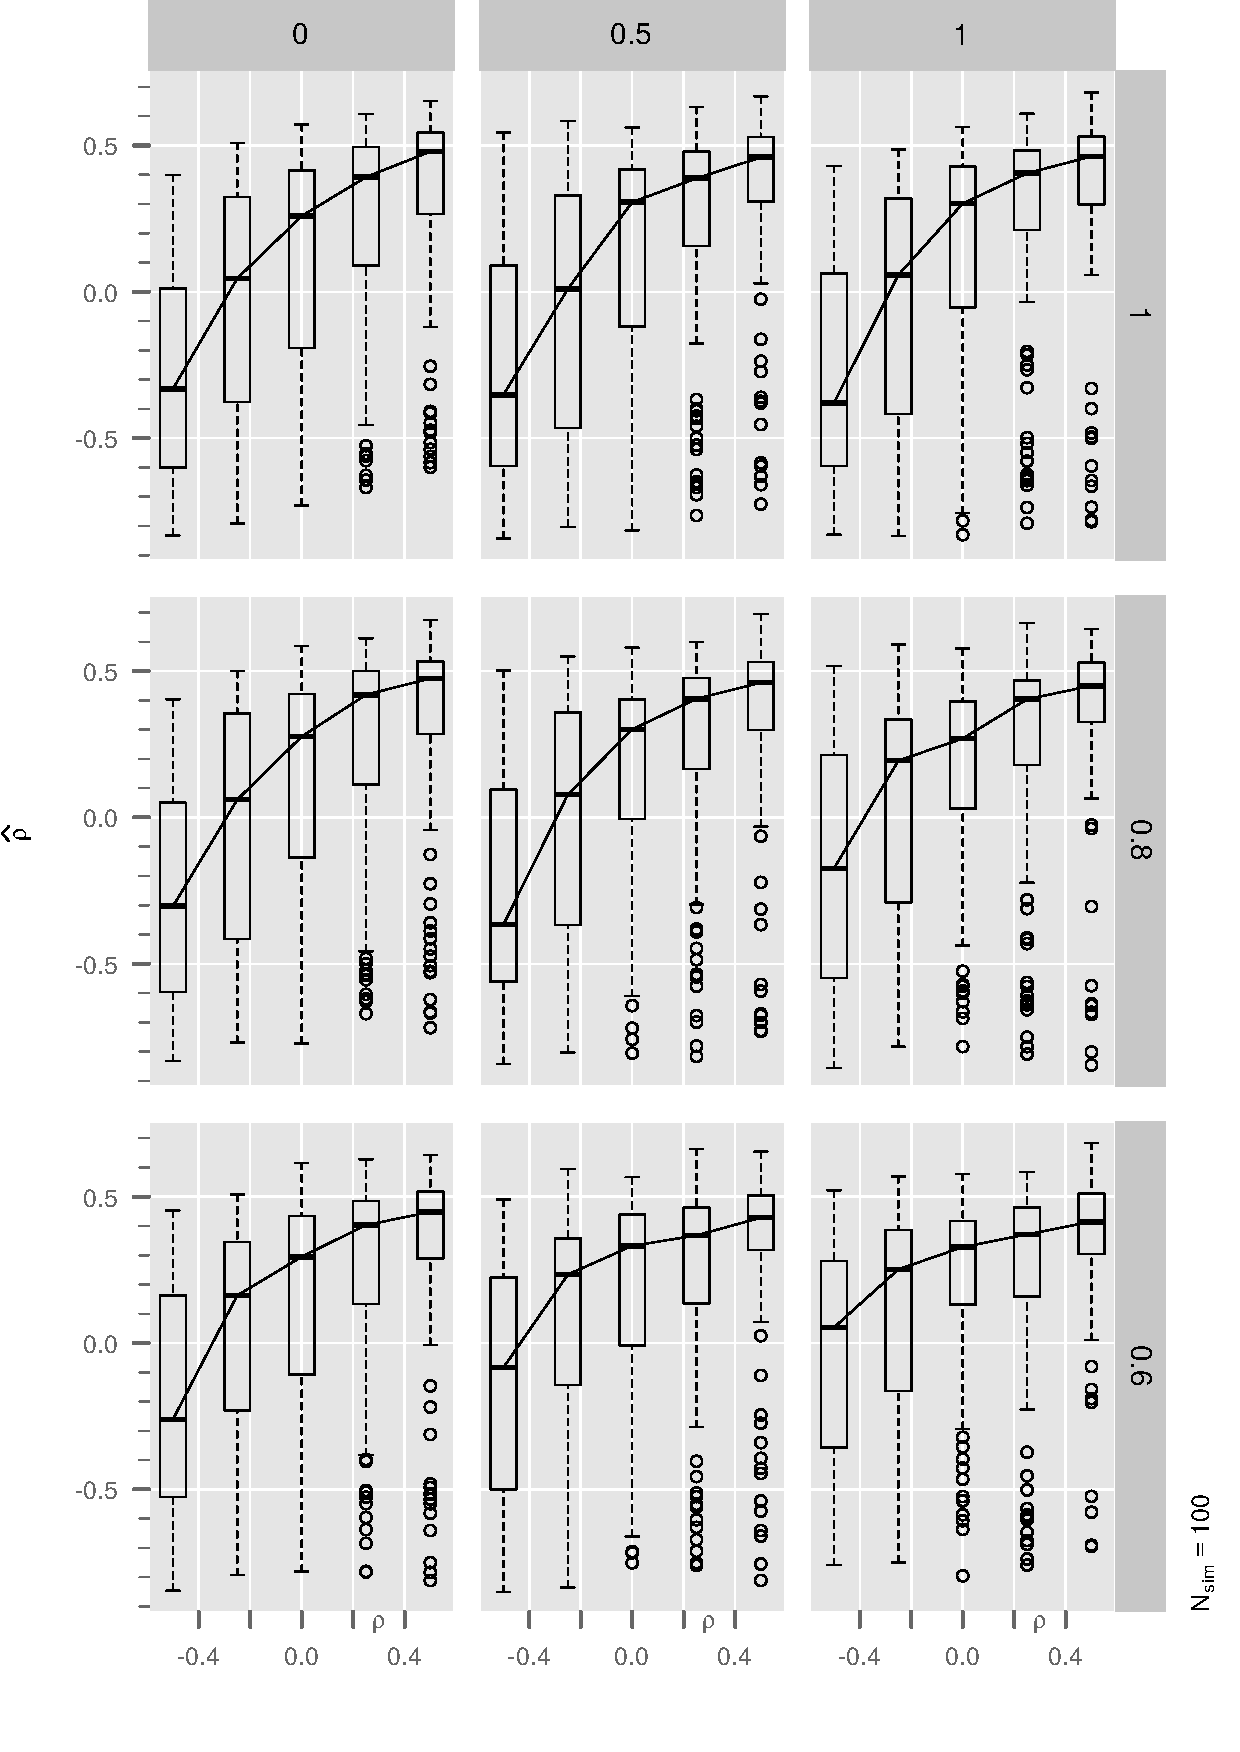
\includegraphics[trim= 0cm 0cm 0cm 11.75cm, clip, scale=0.475]{Figure1/tbl1_n100_rho_mayplot.pdf}
\end{center}

\end{frame}

\begin{frame}{Correlation, n=500 (Density plot)}

\begin{center}
  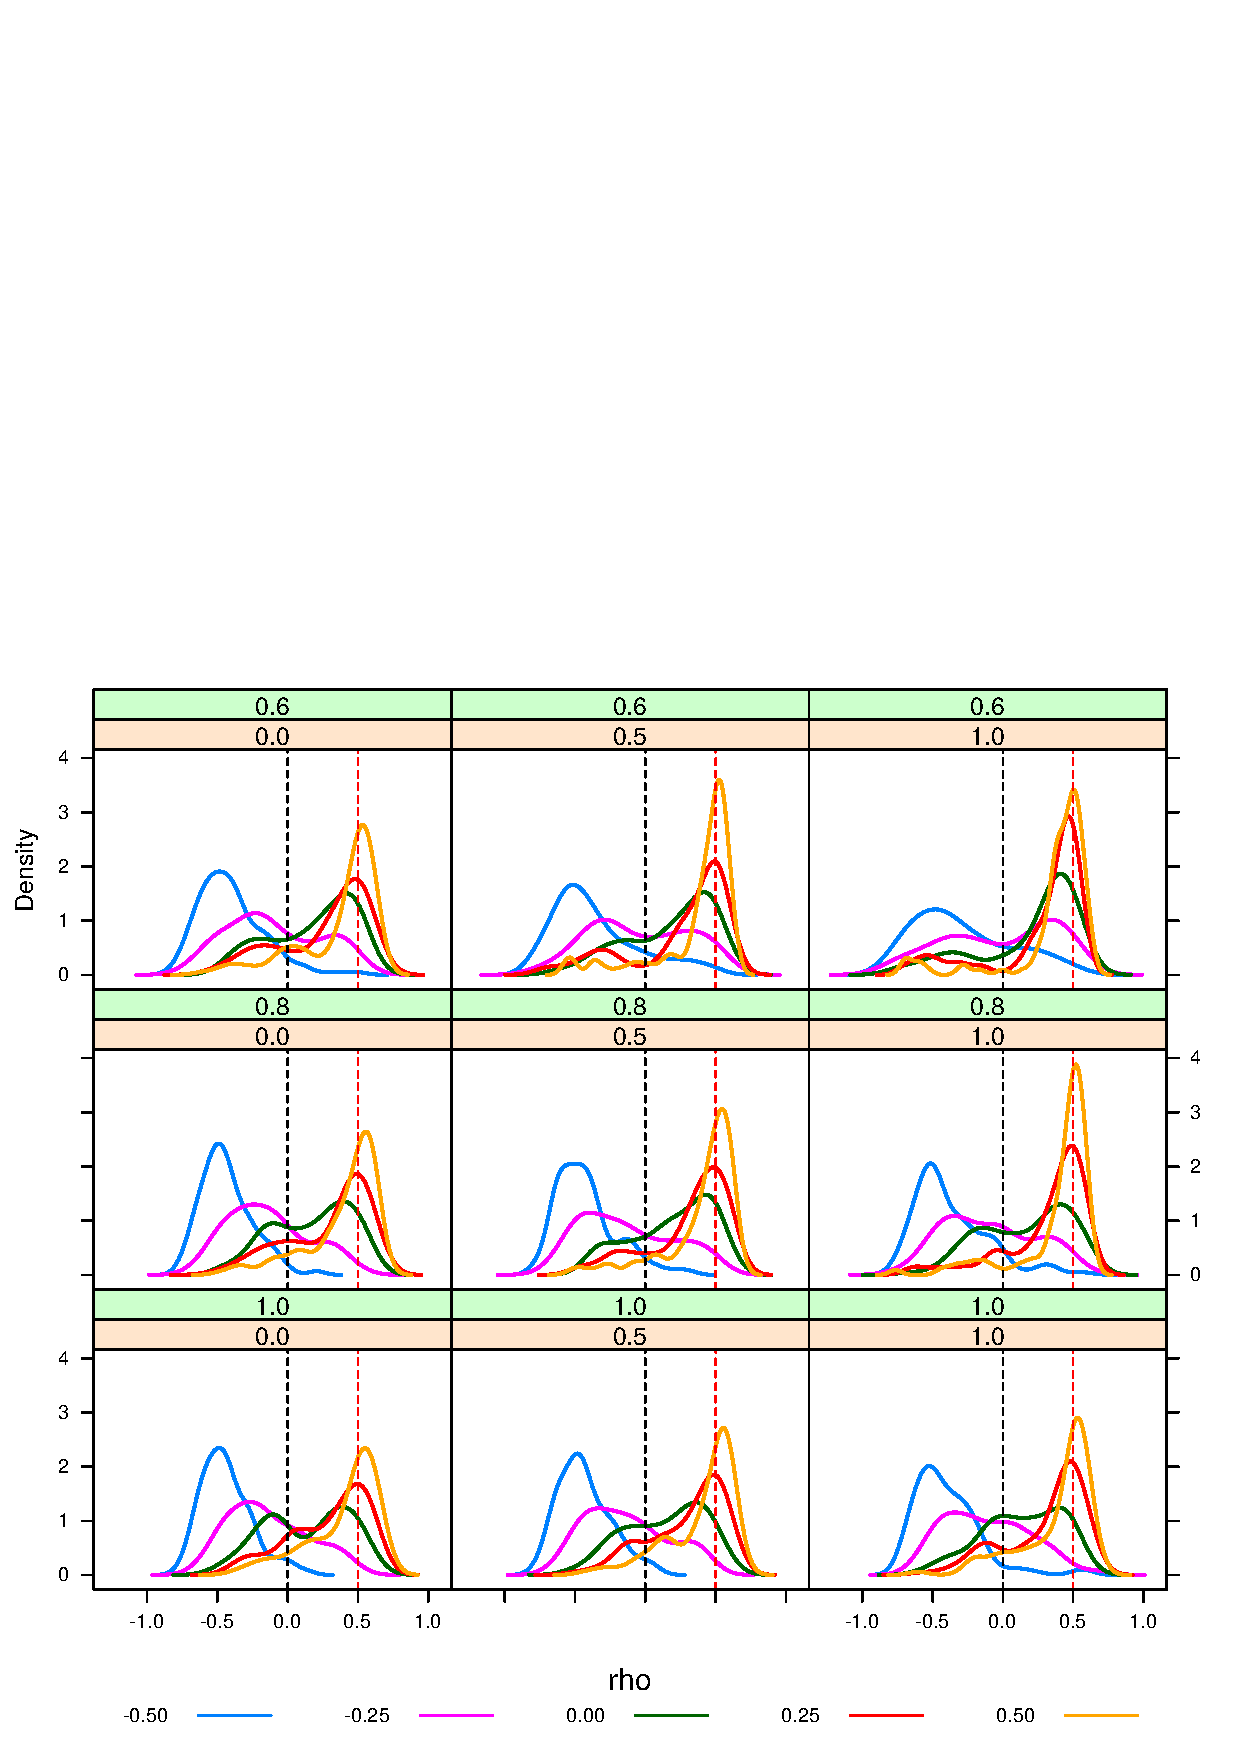
\includegraphics[trim= 0cm 0cm 0cm 11.75cm, clip, scale=0.47]{Figure1/tbl1densityPlot_n500.pdf} % width=1.00\textwidth, clip,, [scale=0.67]
\end{center}

\end{frame}

% ==============================================================================================
\section{{2-sample} estimation of treatment benefit}
\protect\hypertarget{two-samples}{}

\begin{frame}{Treatment Benefit $\hat{\Delta}=\hat{\beta}_{21}$ (n=1000)} % 3b: n=1000
\begin{table}[htbp]
  \centering\scriptsize
  \begin{tabular}{*{2}{l}*{4}{r}}
    \toprule
     & beta12 & \multicolumn{2}{c}{0} & \multicolumn{2}{c}{1} \\
    \cmidrule(lr){3-4} \cmidrule(lr){5-6}
    cs & \( \rho \) \textbar\ deltaTreat & \multicolumn{1}{c}{0} & \multicolumn{1}{c}{0.5} & \multicolumn{1}{c}{0} & \multicolumn{1}{c}{0.5} \\
    \midrule
    1 & -0.5 & -0.00 & 0.50 & 0.00 & 0.51 \\
    & -0.25 & -0.00 & 0.48 & -0.01 & 0.50 \\
    & 0 & 0.00 & 0.46 & 0.00 & 0.50 \\
    & 0.25 & -0.01 & 0.49 & 0.00 & 0.49 \\
    & 0.5 & -0.00 & 0.52 & -0.00 & 0.49 \\ \addlinespace[3pt]
    0.8 & -0.5 & -0.00 & 0.50 & 0.00 & 0.50 \\
    & -0.25 & -0.00 & 0.48 & 0.01 & 0.49 \\
    & 0 & 0.01 & 0.49 & 0.00 & 0.49 \\
    & 0.25 & -0.00 & 0.48 & -0.01 & 0.48 \\
    & 0.5 & -0.01 & 0.51 & 0.01 & 0.51 \\ \addlinespace[3pt]
    0.6 & -0.5 & 0.02 & 0.49 & -0.01 & 0.48 \\
    & -0.25 & -0.02 & 0.52 & -0.00 & 0.48 \\
    & 0 & -0.01 & 0.49 & 0.01 & 0.48 \\
    & 0.25 & 0.02 & 0.49 & 0.01 & 0.50 \\
    & 0.5 & 0.00 & 0.51 & -0.01 & 0.51 \\
    \bottomrule
    \multicolumn{5}{l}{\footnotesize{medians of 100 replicates}} % \multicolumn{4}{l}{\textsuperscript{*}\footnotesize{The footnote}}
  \end{tabular}
%  \caption{b21 TreatDiff estimate: Table 3b, n=1000}
  \label{tab:ft21}
\end{table}

\end{frame}


%\begin{frame}{2-sample: Treatment Benefit, n=1000 (estimates)} % sf x beta12

%\begin{center}
%  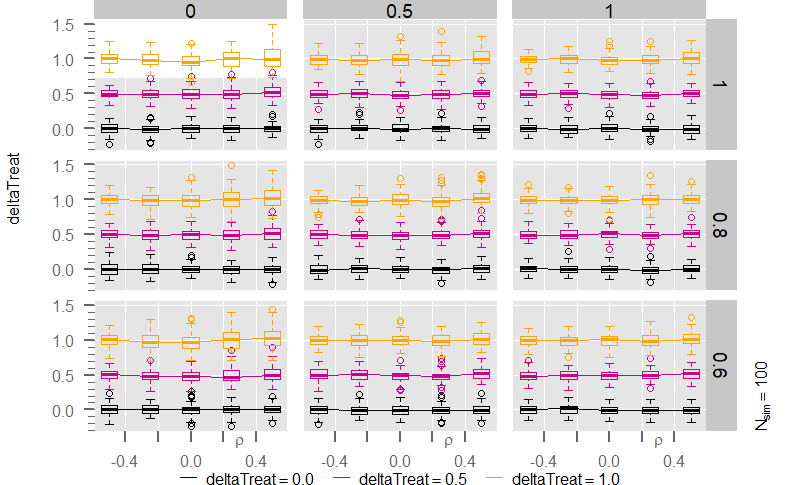
\includegraphics[width=1.00\textwidth]{Figure3/mayplot3-deltaTreat-n1000.png}
%\end{center}

%\end{frame}

%{Treatment Benefit, n=1000, sf=0.6 (density plots)}
%  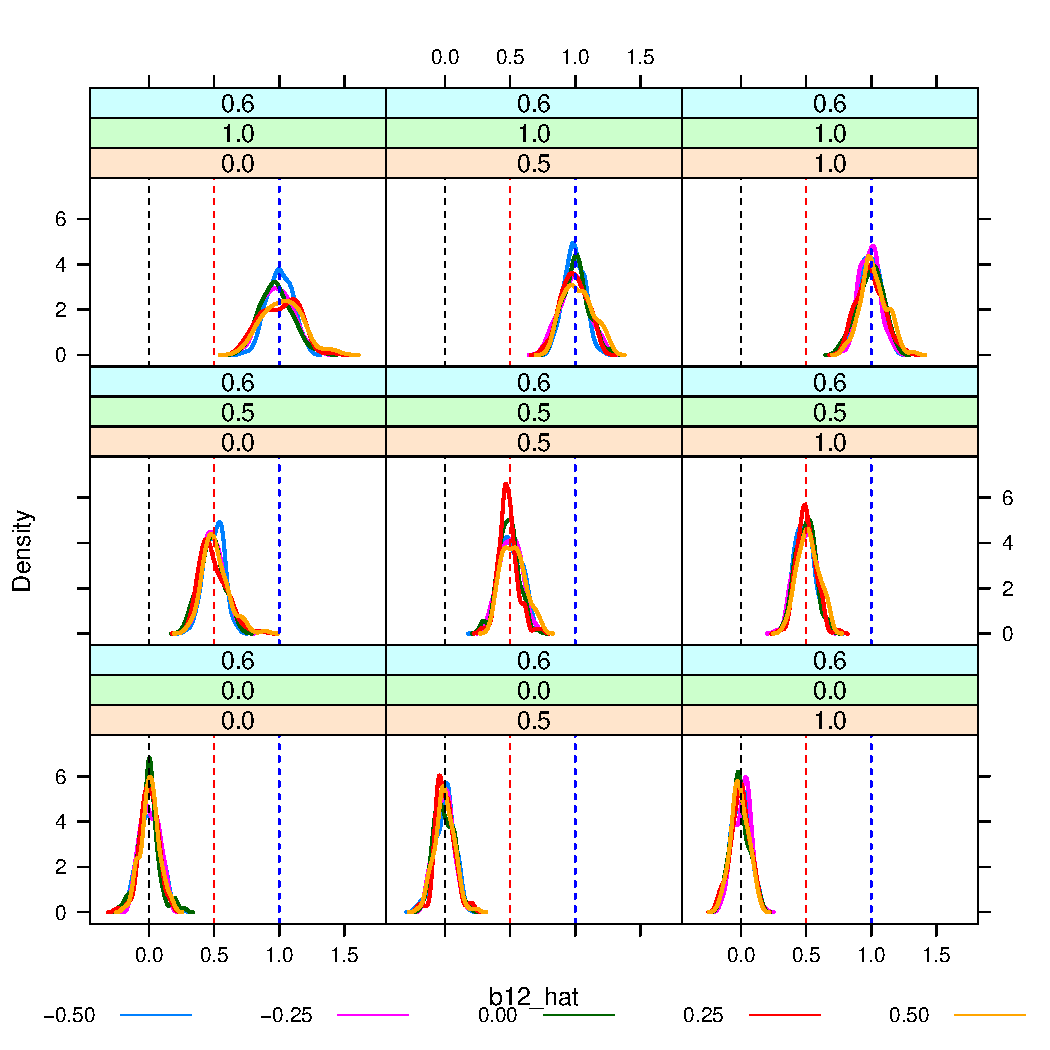
\includegraphics[scale=0.45]{Figure3/tbl3DensityPlots_n1000_003.pdf} % sf=0.6

\begin{frame}{Treatment Benefit, n=100 (estimates)} % sf x beta12

\begin{center}
  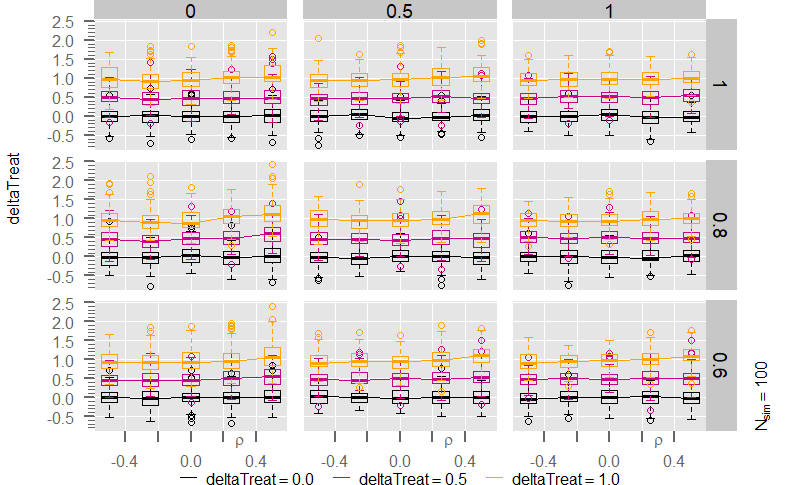
\includegraphics[width=0.95\textwidth]{Figure3/mayplot3-deltaTreat-n100.png}
\end{center}

\end{frame}

%  \includegraphics[width=0.95\textwidth]{Figure3/estimateDifferences2v12.pdf}


%\begin{frame}{2-sample: Treatment difference: BNC estimate  vs survreg coef ($\rho=0$)}

%\begin{center}
%  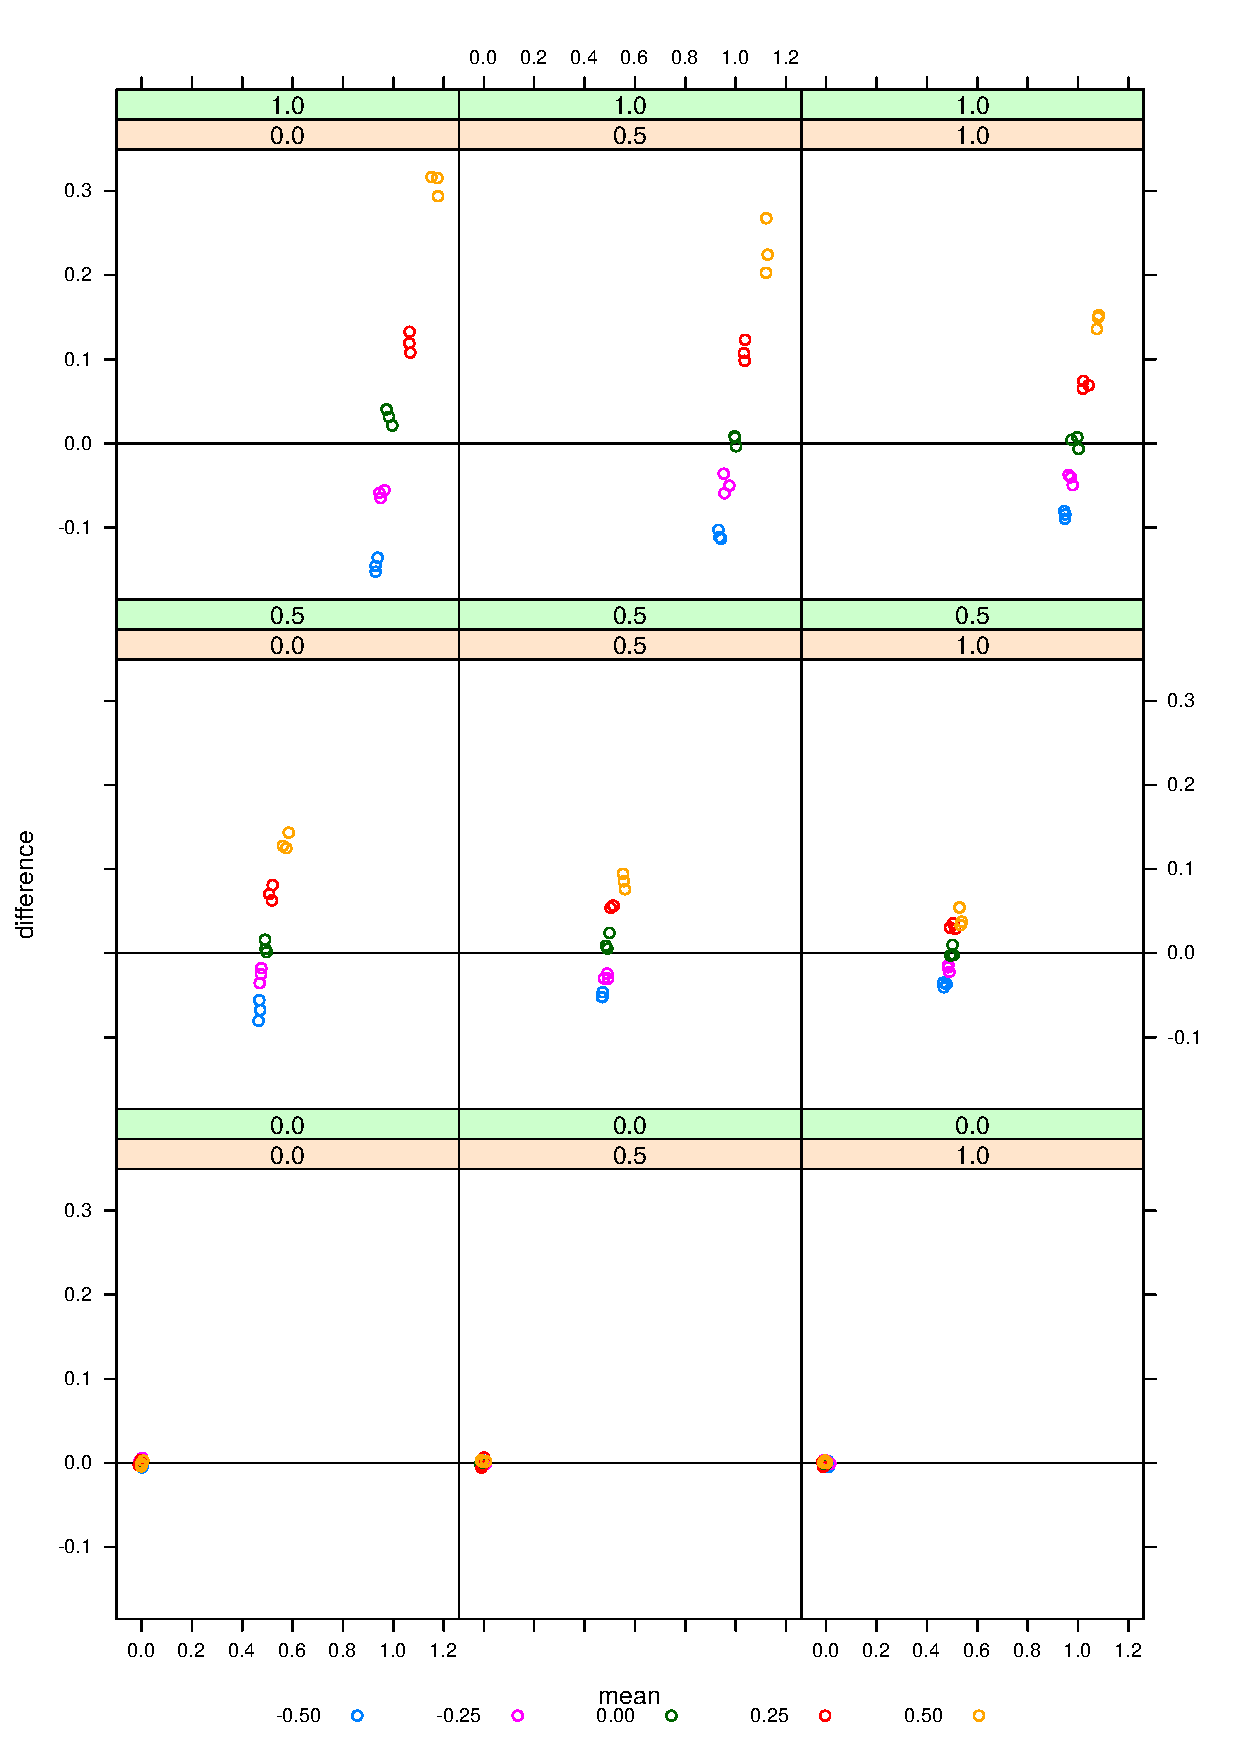
\includegraphics[height=0.95\textheight,width=0.95\textwidth]{%
%  Figure3/estimateDifferences2vs12v2.pdf%
%  }
%\end{center}

%\end{frame}


\begin{frame}{Treatment Benefit, n=1000, sf=0.6 (density plots)}

\begin{center}
  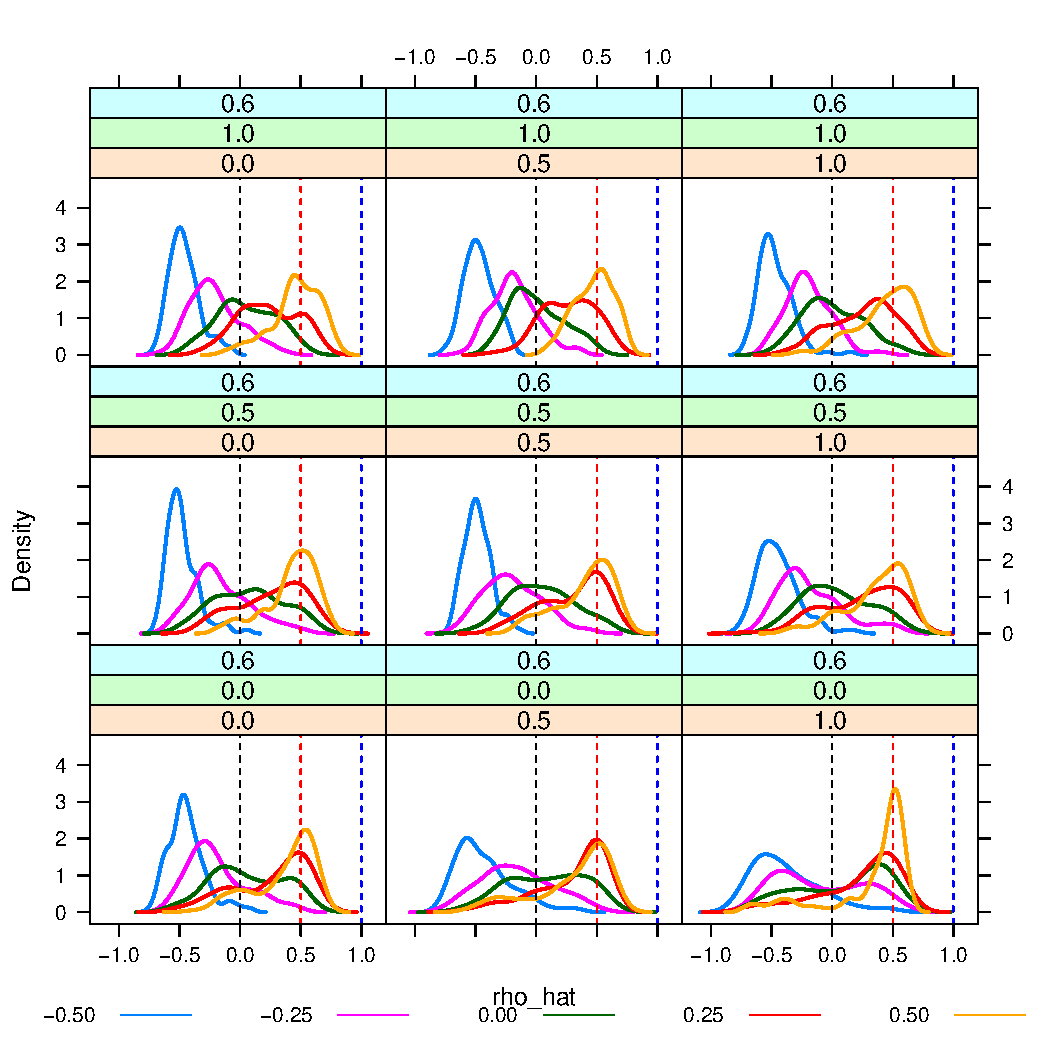
\includegraphics[scale=0.45]{Figure3/tbl3DensityPlots_rho_n1000_003.pdf} % sf=0.6
\end{center}

\end{frame}


